%===============METODOLOGÍA==================
%\section{Metodología}
%Para la realización del trabajo terminal se seguirá la metodología descrita por el Modelo en V ya que ofrece una visión detallada de los diversos pasos e interacciones relacionados con el proceso de desarrollo y puede considerarse como un flujo de trabajo comúnmente utilizado. \cite{perez2006V} \\
%
%En la Figura \ref{fig:IntroduccionMetodologia} se muestran las principales actividades abordadas por el método. Convencionalmente, el lado izquierdo del modelo representa las fases del diseño del sistema, mientras que el lado derecho representa las fases de validación y verificación del sistema. \\
%
%\begin{figure}[htbp!]
%	\centering
%	\fbox{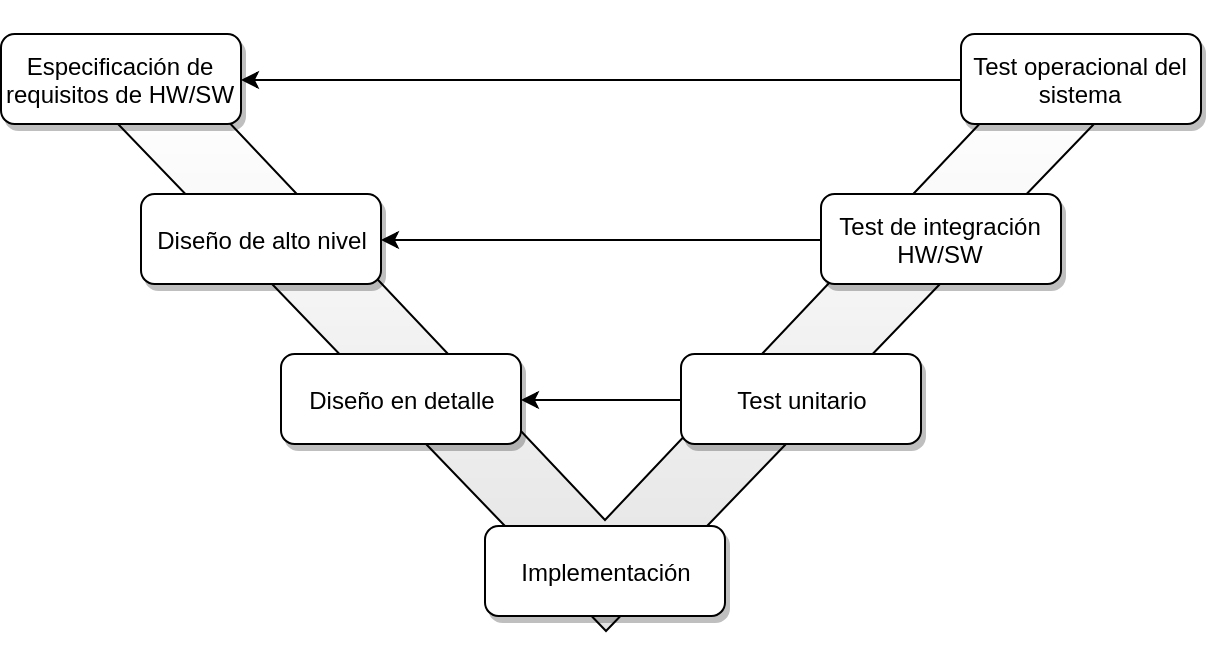
\includegraphics[width=\textwidth]{DisenoEstructura/imagenes/metodologiaV.png}}
%	\caption{Fases del Modelo en V.}
%	\label{fig:IntroduccionMetodologia}
%\end{figure}
%
%El desarrollo se llevará a cabo de la siguiente manera: \\
%
%Partiendo de la \textbf{Especificación de requisitos HW/SW}, se pretende definir y documentar los diferentes requerimientos del sistema a implementar, seguido de un diseño global o \textbf{Diseño de alto nivel} que permitirá obtener una visión general del sistema identificando las funciones que deberá cumplir y asignarlas a los diferentes componentes, ya sea de HW o SW. El \textbf{Diseño en detalle} consiste en detallar cada elemento que consituyen los componentes del sistema global, en donde se pretende especificar el diseño del sistema embebido con los componentes a implementar y de la aplicación móvil, seguida de la \textbf{Implementación} de cada uno de ellos, en donde los módulos de SW son desarrollados e integrados con el HW. En el \textbf{Test unitario} se verificará cada módulo de HW y SW de manera individual, en donde se depurará cada uno de ellos hasta obtener el resultado deseado. En la \textbf{Test de integración HW/SW} se acoplan los diferentes módulos del sistema para verificar su funcionamiento en conjunto y finalmente en el \textbf{Test operacional del sistema} se realizarán las últimas pruebas en un escenario real y así validar si los resultados obtenidos cumplen con los requerimientos. \\